\chapter{Progettazione}

Nella fase di progettazione, si sono fatte alcune assunzioni sull'ambiente, sul drone e sulle altre entità coinvolte durante la fase di simulazione.
In particolare, tali assunzioni riguardano le caratteristiche principali dell'ambiente e delle entità in esso coinvolte.

\section{Progettazione dell'ambiente}

L'ambiente che viene preso in esame dipende dallo scenario considerato per la simulazione della missione.
Esso rappresenta un'area bidimensionale strutturata e limitata, in cui lo spazio ed il tempo risultano entrambi discretizzati.

Lo spazio è simulato attraverso una griglia di \textit{NxM} celle quadrate, dette \textit{patch}, di lato \textit{S}. 
Il tempo è discretizzato in una sequenza di intervalli temporali di durata \textit{T} detti \textit{tick} definiti come:
\begin{equation*}
    t_0 + T, t_0 + 2T, \dots, t_0 + NT
\end{equation*}

L'ambiente simulato contiene i seguenti elementi: 
\begin{itemize}
    \item \textit{Droni};
    \item \textit{Target};
    \item \textit{Ostacoli};
    \item \textit{Feromoni digitali};
\end{itemize}

\begin{figure}[H] 
    \begin{center}
    \makebox[\textwidth]{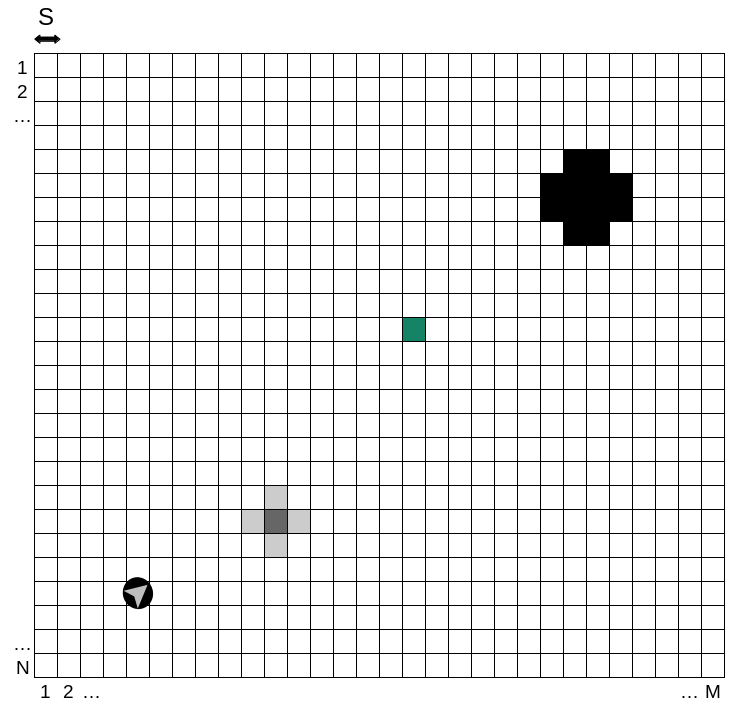
\includegraphics[width=0.5\paperwidth]{img/elementi_ambiente.png}}
    \end{center}
    \caption{Definizione dell'ambiente simulato}
    \label{elementi_ambiente}
\end{figure}



Nel simulatore implementato, si sono assunti i seguenti valori:
\begin{itemize}
    \item S = 1 metro;
    \item T = 1 secondo; 
\end{itemize}